\documentclass[12pt]{article}
\usepackage[a4paper]{geometry}
\usepackage{fullpage}
\usepackage[T1]{fontenc}
\usepackage[utf8]{inputenc}
\usepackage{graphicx}
\usepackage{mathpazo}
\pagenumbering{gobble}
\usepackage{siunitx}
\sisetup{output-decimal-marker = {,}}
\usepackage{amsmath}
\usepackage{esdiff}
\usepackage[spanish]{babel}
\newcommand{\laplace}[1]{\mathbf{#1}(\mathbf{s})}
\newcommand{\slp}{\mathbf{s}}

\begin{document}

\title{\textsc{Teoría de Circuitos III}\\Prueba BT2}

\date{25 de octubre de  2018\\\small{Los resultados se publicarán el día 31 de octubre.\\La revisión del examen se realizará en horario de tutoría los días 6, 7 y 8 de noviembre.}}

\maketitle

El interruptor del circuito de la figura ha permanecido abierto un tiempo elevado, y se cierra en $t = 0$. En estas condiciones debe realizar el siguiente itinerario:

\begin{enumerate}
\item (\textbf{0,5p.}) Determinar las condiciones iniciales de las variables $u_C(0^+)$, $i_L(0^+)$, $i_R(0^+)$.
\item (\textbf{0,5p.}) Determinar los valores en régimen permanente de las variables $u_C(\infty)$, $i_L(\infty)$, $i_R(\infty)$.
\item (\textbf{4p.}) Dibujar el circuito en el dominio de Laplace para $t > 0$, y resolverlo para obtener las expresiones analíticas de $\laplace{I_L}$, $\laplace{U_C}$, $\laplace{I_R}$.
\item (\textbf{1p.}) Comprobar mediante los teoremas de valor inicial y valor final que las expresiones anteriores se ajustan a los resultados de los apartados 1 y 2.

\item (\textbf{1p.}) A partir de las expresiones obtenidas en el apartado 3, indique de forma razonada el tipo de transitorio existente en el circuito.

\item (\textbf{3p.}) Expresión en el dominio del tiempo de la variable $i_R(t)$.
\end{enumerate}

\begin{minipage}{0.3\textwidth}
Datos:
\begin{align*}
  E_g &= \SI{500}{\volt}\\
  R_{L}&= \SI{10}{\ohm}\\
  L &= \SI{200}{\milli\henry}\\
  C &= \SI{100}{\milli\farad}\\
  R &= \SI{1}{\ohm}
\end{align*}
\end{minipage}
\begin{minipage}{0.7\textwidth}
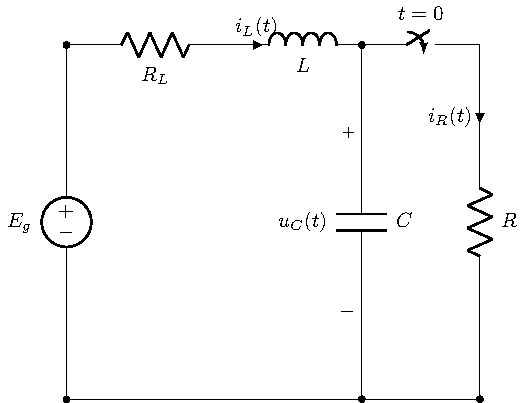
\includegraphics{figs/E2_circuito.pdf}
\end{minipage}

\clearpage

\subsection*{Solución}

\begin{enumerate}

\item

  La siguiente figura representa el circuito para $t = 0^-$.

  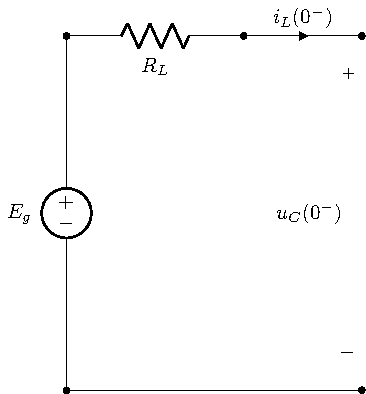
\includegraphics{figs/E2_t0.pdf}

  En este circuito obtenemos:

\begin{align*}
  i_L(0^-) &= \SI{0}{\ampere}\\
  u_c(0^-) &= \SI{500}{\volt}
\end{align*}

Mediante las condiciones de continuidad, obtenemos:

\begin{align*}
  i_L(0^+) &= \SI{0}{\ampere}\\
  u_c(0^+) &= \SI{500}{\volt}\\
  i_R(0^+) &= u_c(0^+)/R = \SI{500}{\ampere}
\end{align*}

\item


  La siguiente figura representa el circuito para $t \to \infty$.

  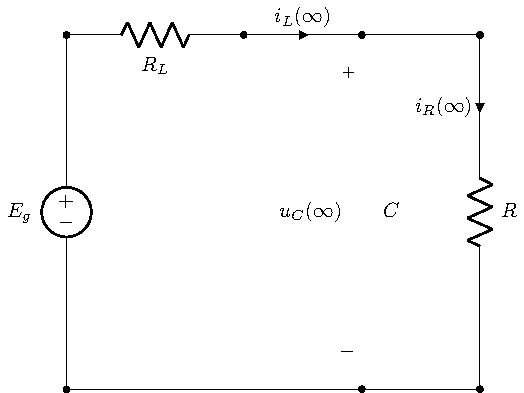
\includegraphics{figs/E2_permanente.pdf}

  En este circuito obtenemos:
  \begin{align*}
    i_L(\infty) &= \frac{E_g}{R + R_L} = \SI{45.45}{\ampere}\\
    u_C(\infty) &= \frac{R \cdot Eg}{R + R_L} = \SI{45.45}{\volt}\\
    i_R(\infty) &= i_L(\infty)
  \end{align*}

\item

  La siguiente figura representa el circuito en el dominio de Laplace.

  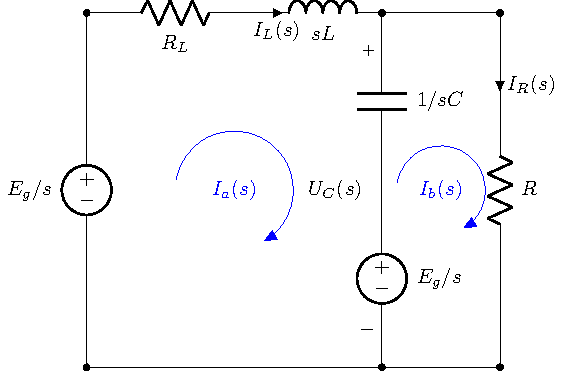
\includegraphics{figs/E2_laplace.pdf}

  En este circuito se han indicado las corrientes de malla que se relacionan con las variables solicitadas:
  \begin{align*}
    \laplace{I_L} &= \laplace{I_a}\\
    \laplace{I_R} &= \laplace{I_b}\\
    \laplace{U_C} &= R \laplace{I_R} = \laplace{I_R}
  \end{align*}
  
  Las ecuaciones de las mallas son:

  \[
    \left(
    \begin{array}{cc}
      10 + 0,2\slp + 10/\slp & -10/\slp\\
      -10/\slp & 10/\slp + 1
    \end{array}
  \right)
  \cdot
  \left(
    \begin{array}{c}
      \laplace{I_a}\\
      \laplace{I_b}
    \end{array}
  \right)
  =
  \left(
    \begin{array}{c}
      0\\
      Eg/\slp
    \end{array}
  \right)
  \]

  Resolviendo el sistema y empleando las relaciones anteriores se obtiene:

  \begin{align*}
    \laplace{I_L} &= \frac{\num{25e3}}{\slp(\slp^2 + 60\slp + 550)}\\
    \laplace{I_R} &= 500 \frac{\slp^2 + 50\slp + 50}{\slp(\slp^2 + 60\slp + 550)}\\
    \laplace{U_C} &= 500 \frac{\slp^2 + 50 \slp + 50}{\slp(\slp^2 + 60\slp + 550)}
  \end{align*}



\item

  Los resultados del teorema de valor inicial son:

  \begin{align*}
    \lim_{s \to \infty} \slp \laplace{I_L} = i_L(0^+) &= \SI{0}{\ampere}\\
    \lim_{s \to \infty} \slp \laplace{I_R} = i_R(0^+) &= \SI{500}{\ampere}\\
    \lim_{s \to \infty} \slp \laplace{U_C} = u_c(0^+) &= \SI{500}{\volt}\\
  \end{align*}

  Los resultados del teorema de valor final son:

  \begin{align*}
    \lim_{s \to 0} \slp \laplace{I_L} = i_L(\infty) &= \SI{45.45}{\ampere}\\
    \lim_{s \to 0} \slp \laplace{I_R} = i_R(\infty) &= \SI{45.45}{\ampere}\\
    \lim_{s \to 0} \slp \laplace{U_C} = u_C(\infty) &= \SI{45.45}{\volt}\\
  \end{align*}

  Estos resultados corresponden con los obtenidos en los apartados 1 y 2.
\item

  Las raíces del denominador son:

  \begin{align*}
    \slp_1 &= 0\\
    \slp_2 &= -48.71\\
    \slp_3 &= -11.29
  \end{align*}

  Teniendo en cuenta que la fuente del sistema es $E_g/\slp$, la primera raíz corresponde a la respuesta forzada. Las otras dos raíces corresponden a los polos del sistema y, por tanto, a la respuesta natural. Se trata de dos raíces reales y distintas, lo que implica un transitorio sobreamortiguado.

  Otra forma de llegar a la misma conclusión es tener en cuenta que, al tratarse de un circuito de segundo orden, el polinomio debe ser de la forma $\slp^2 + 2\alpha\slp + \omega_o^2$. Por tanto,

  \begin{align*}
    \alpha &= 30\\
    \omega_o&= 23.45\\
  \end{align*}

  Dado que $\alpha > \omega_o$, se trata de un transitorio sobreamortiguado con exponentes $\slp_1 = -\alpha - \sqrt{\alpha^2 - \omega_o^2} = -48.71$ y $\slp_2 = -\alpha + \sqrt{\alpha^2 - \omega_o^2} = -11.29$.

\item

  Desarrollamos la expresión $\laplace{I_R}$ en fracciones parciales:

  \[
    \laplace{I_R} = 500 \frac{\slp^2 + 50\slp + 50}{\slp(\slp^2 + 60\slp + 550)} = \frac{A}{\slp} + \frac{B}{\slp + 48.71} + \frac{C}{\slp+11.29}
  \]

  Para determinar los tres coeficientes empleamos las siguientes expresiones:
  \begin{align*}
    A &= \left. \slp \laplace{I_R}\right|_{\slp = 0} = 45.45\\
    B &= \left. (\slp + 48.71) \laplace{I_R}\right|_{\slp = -48.71} = -3.52\\
    C &= \left. (\slp + 11.29) \laplace{I_R}\right|_{\slp = -11.29} = 458.06
  \end{align*}

  Consecuentemente, la expresión de la corriente por la resistencia para $t > 0$ es:

  \[
    i_R(t) = 45.45 -3.52 e^{-48.71 t} + 458.06 e^{-11.29 t}    
  \]

  Tal y como se anticipó anteriormente, se trata de un transitorio sobreamortiguado que comienza en $\SI{500}{\ampere}$ y tiende a $\SI{45.45}{\ampere}$.

  La siguiente figura muestra el resultado gráfico de la simulación de este circuito en Qucs, representando la evolución temporal de esta señal.

  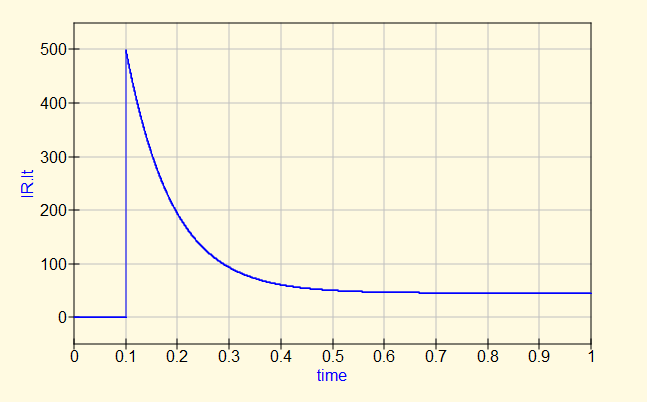
\includegraphics[width=\textwidth]{figs/simulaLaplace.png}

\end{enumerate}

\end{document}

% Local Variables:
% ispell-local-dictionary: "castellano"
% End:

